%
% file: localoperator.tex
% author: Victor Brena
% description: Briefly describes properties of the local operator.
%

\chapter{Uncoupled Flow Failure State Reasoning}
\label{app:app05}

\initial{S}imilarly to FFIP analysis, several initiating events are considered. For each function on the cutsets path, a FFIP analysis is carried to understand the impact on the nominal flow paths. Then, a UFFSR analysis is performed to compute potential new cutsets. The loss of the function {Channel - Guide - Rotate}, which connect the flow \textit{Material - Gas} with \textit{Energy - Mechanical} is propagated on figure~\ref{fig:ffip2}, and a UFFSR analysis graphical example is shown on figure~\ref{fig:uffsr1}. This is equivalent to the loss of the turbines in a RBD, and, in a UFFSR analysis, the explosion of the turbine. Figure~\ref{fig:uffsr2} shows the same event, with an arrestor function (green hexagon) considered on the way (a thick concrete wall in this case).

As in FFIP, two critical functions are defined. These functions are the one that are critical to the system reliability (electricity generation) and the system risks (preventing a core meltdown).

\begin{figure}[t]
\centering
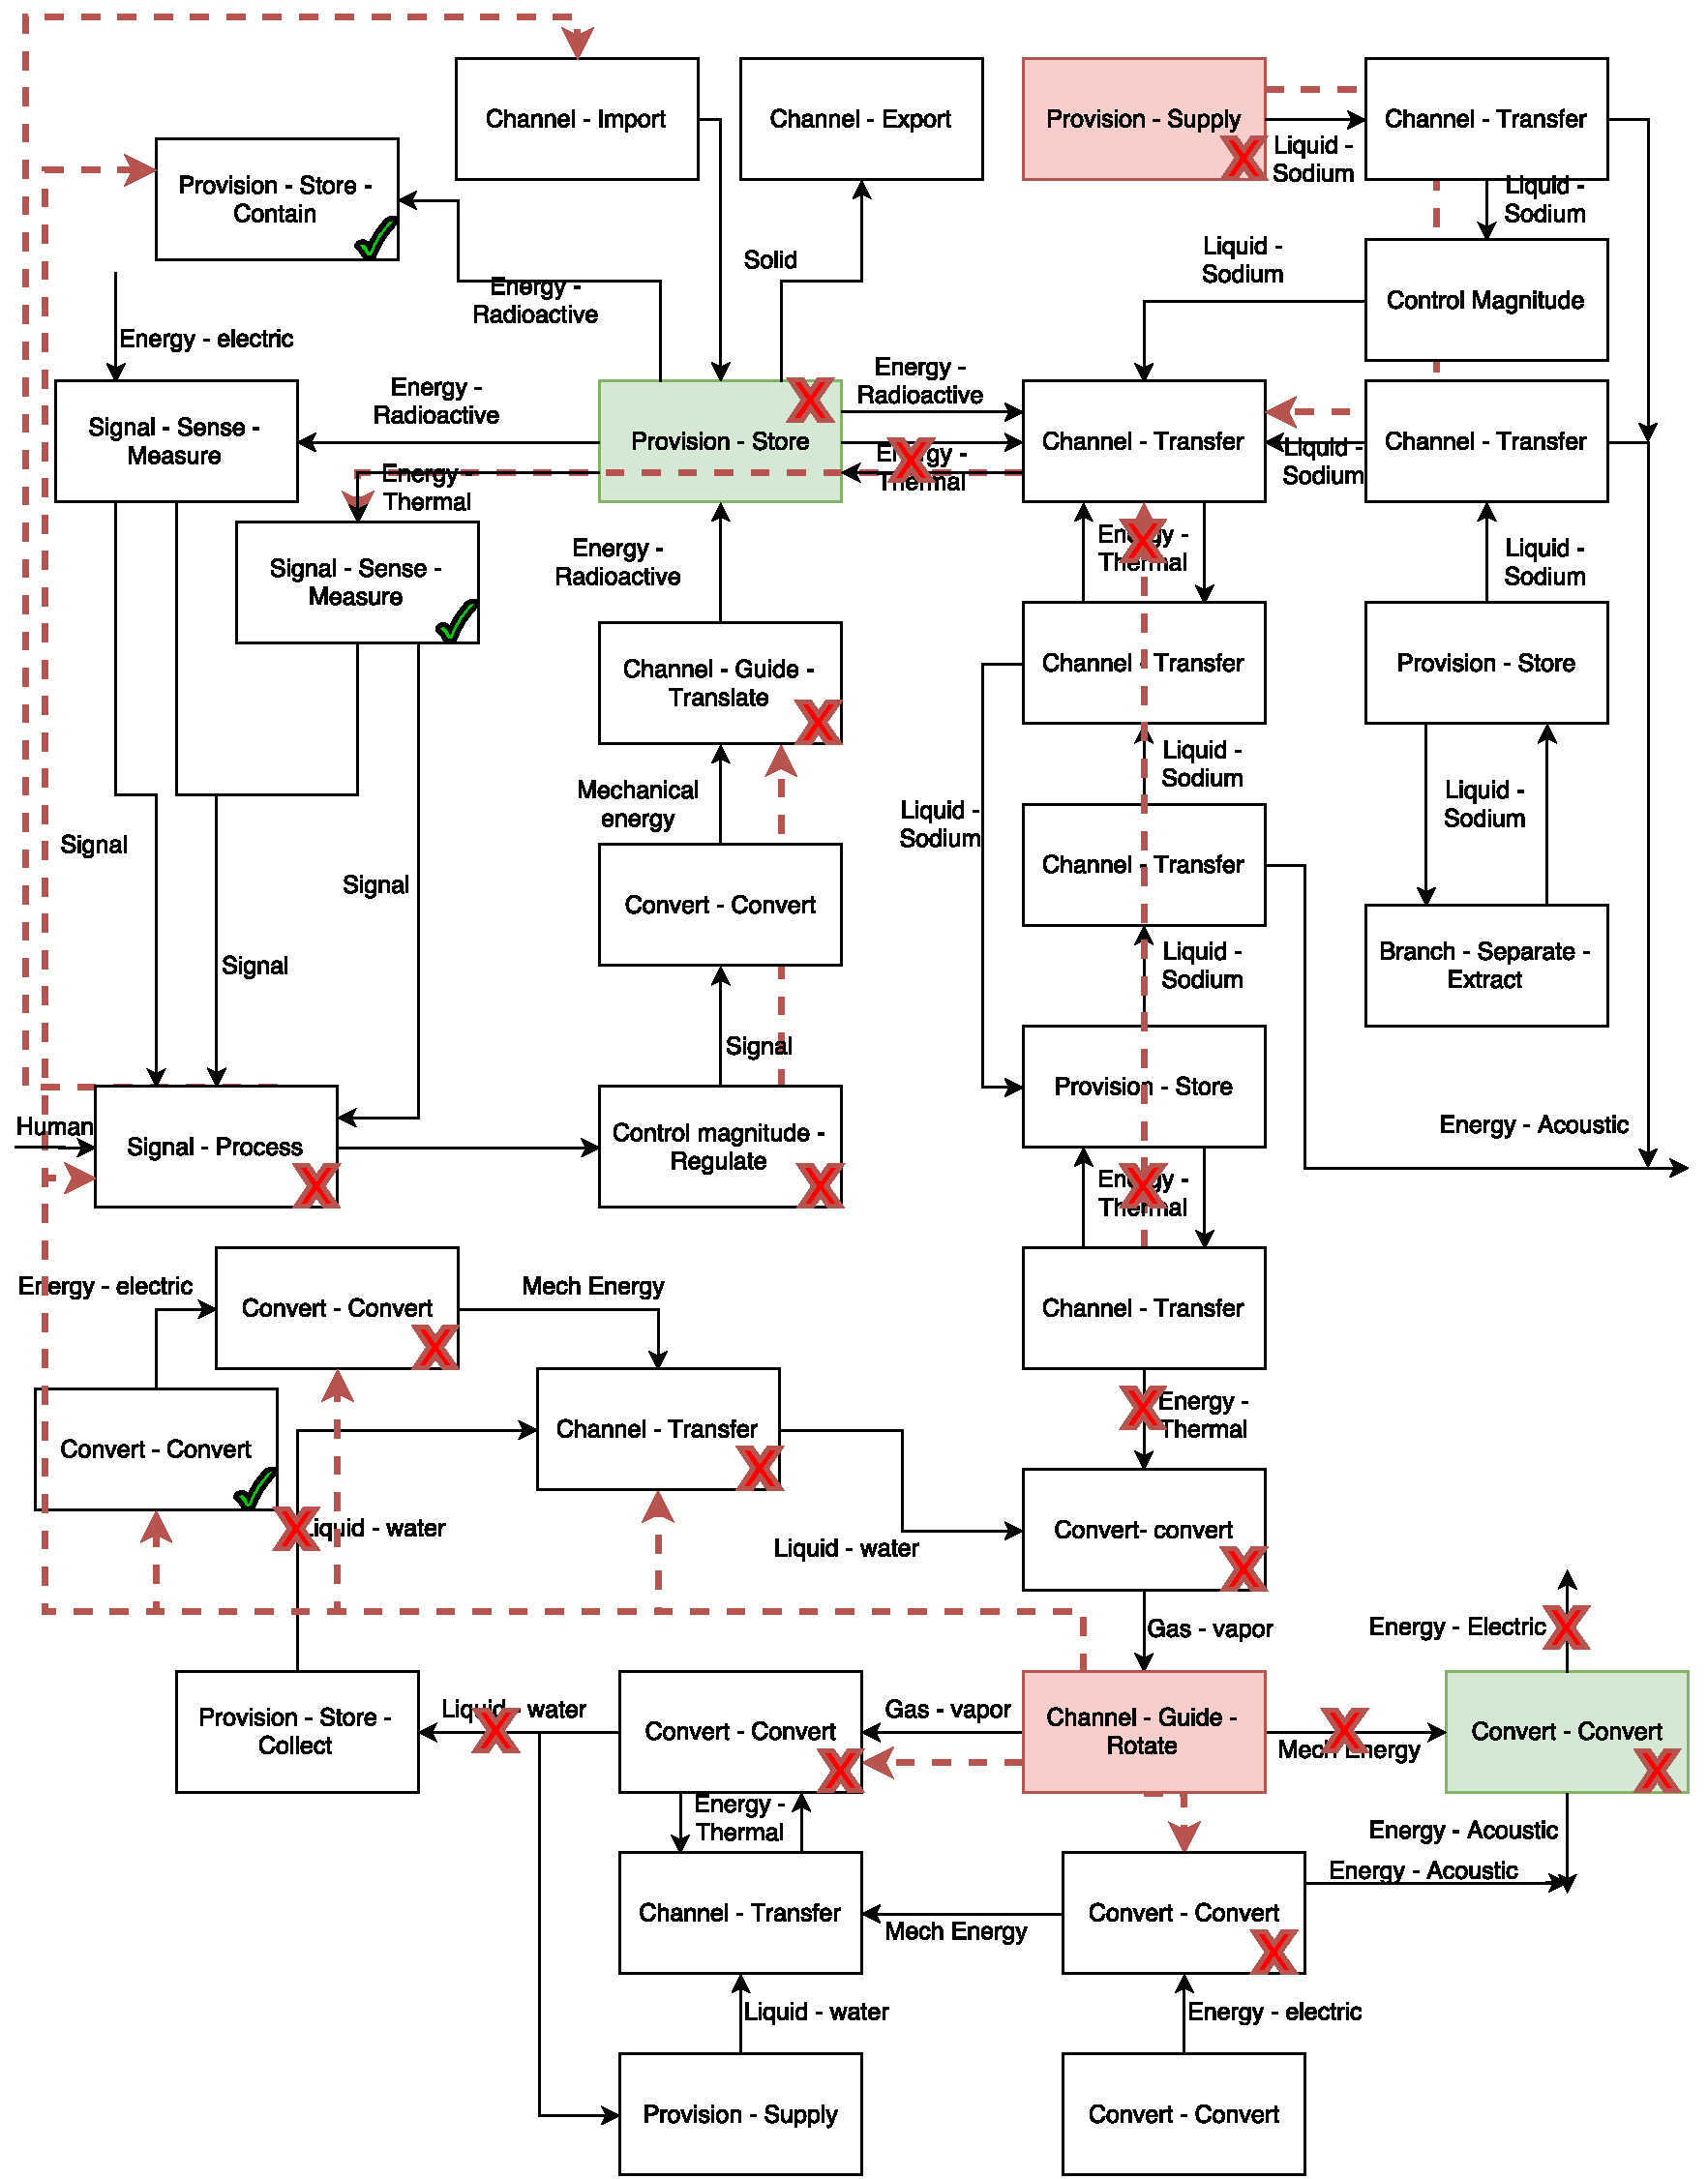
\includegraphics[scale=.55]{fig0e/UFFSR_1}
\caption{UFFSR - Initiating event: Turbine explosion - Secondary event: Loss of sodium supply for the SIS}
\label{fig:uffsr1}
\end{figure}

\begin{figure}[t]
\centering
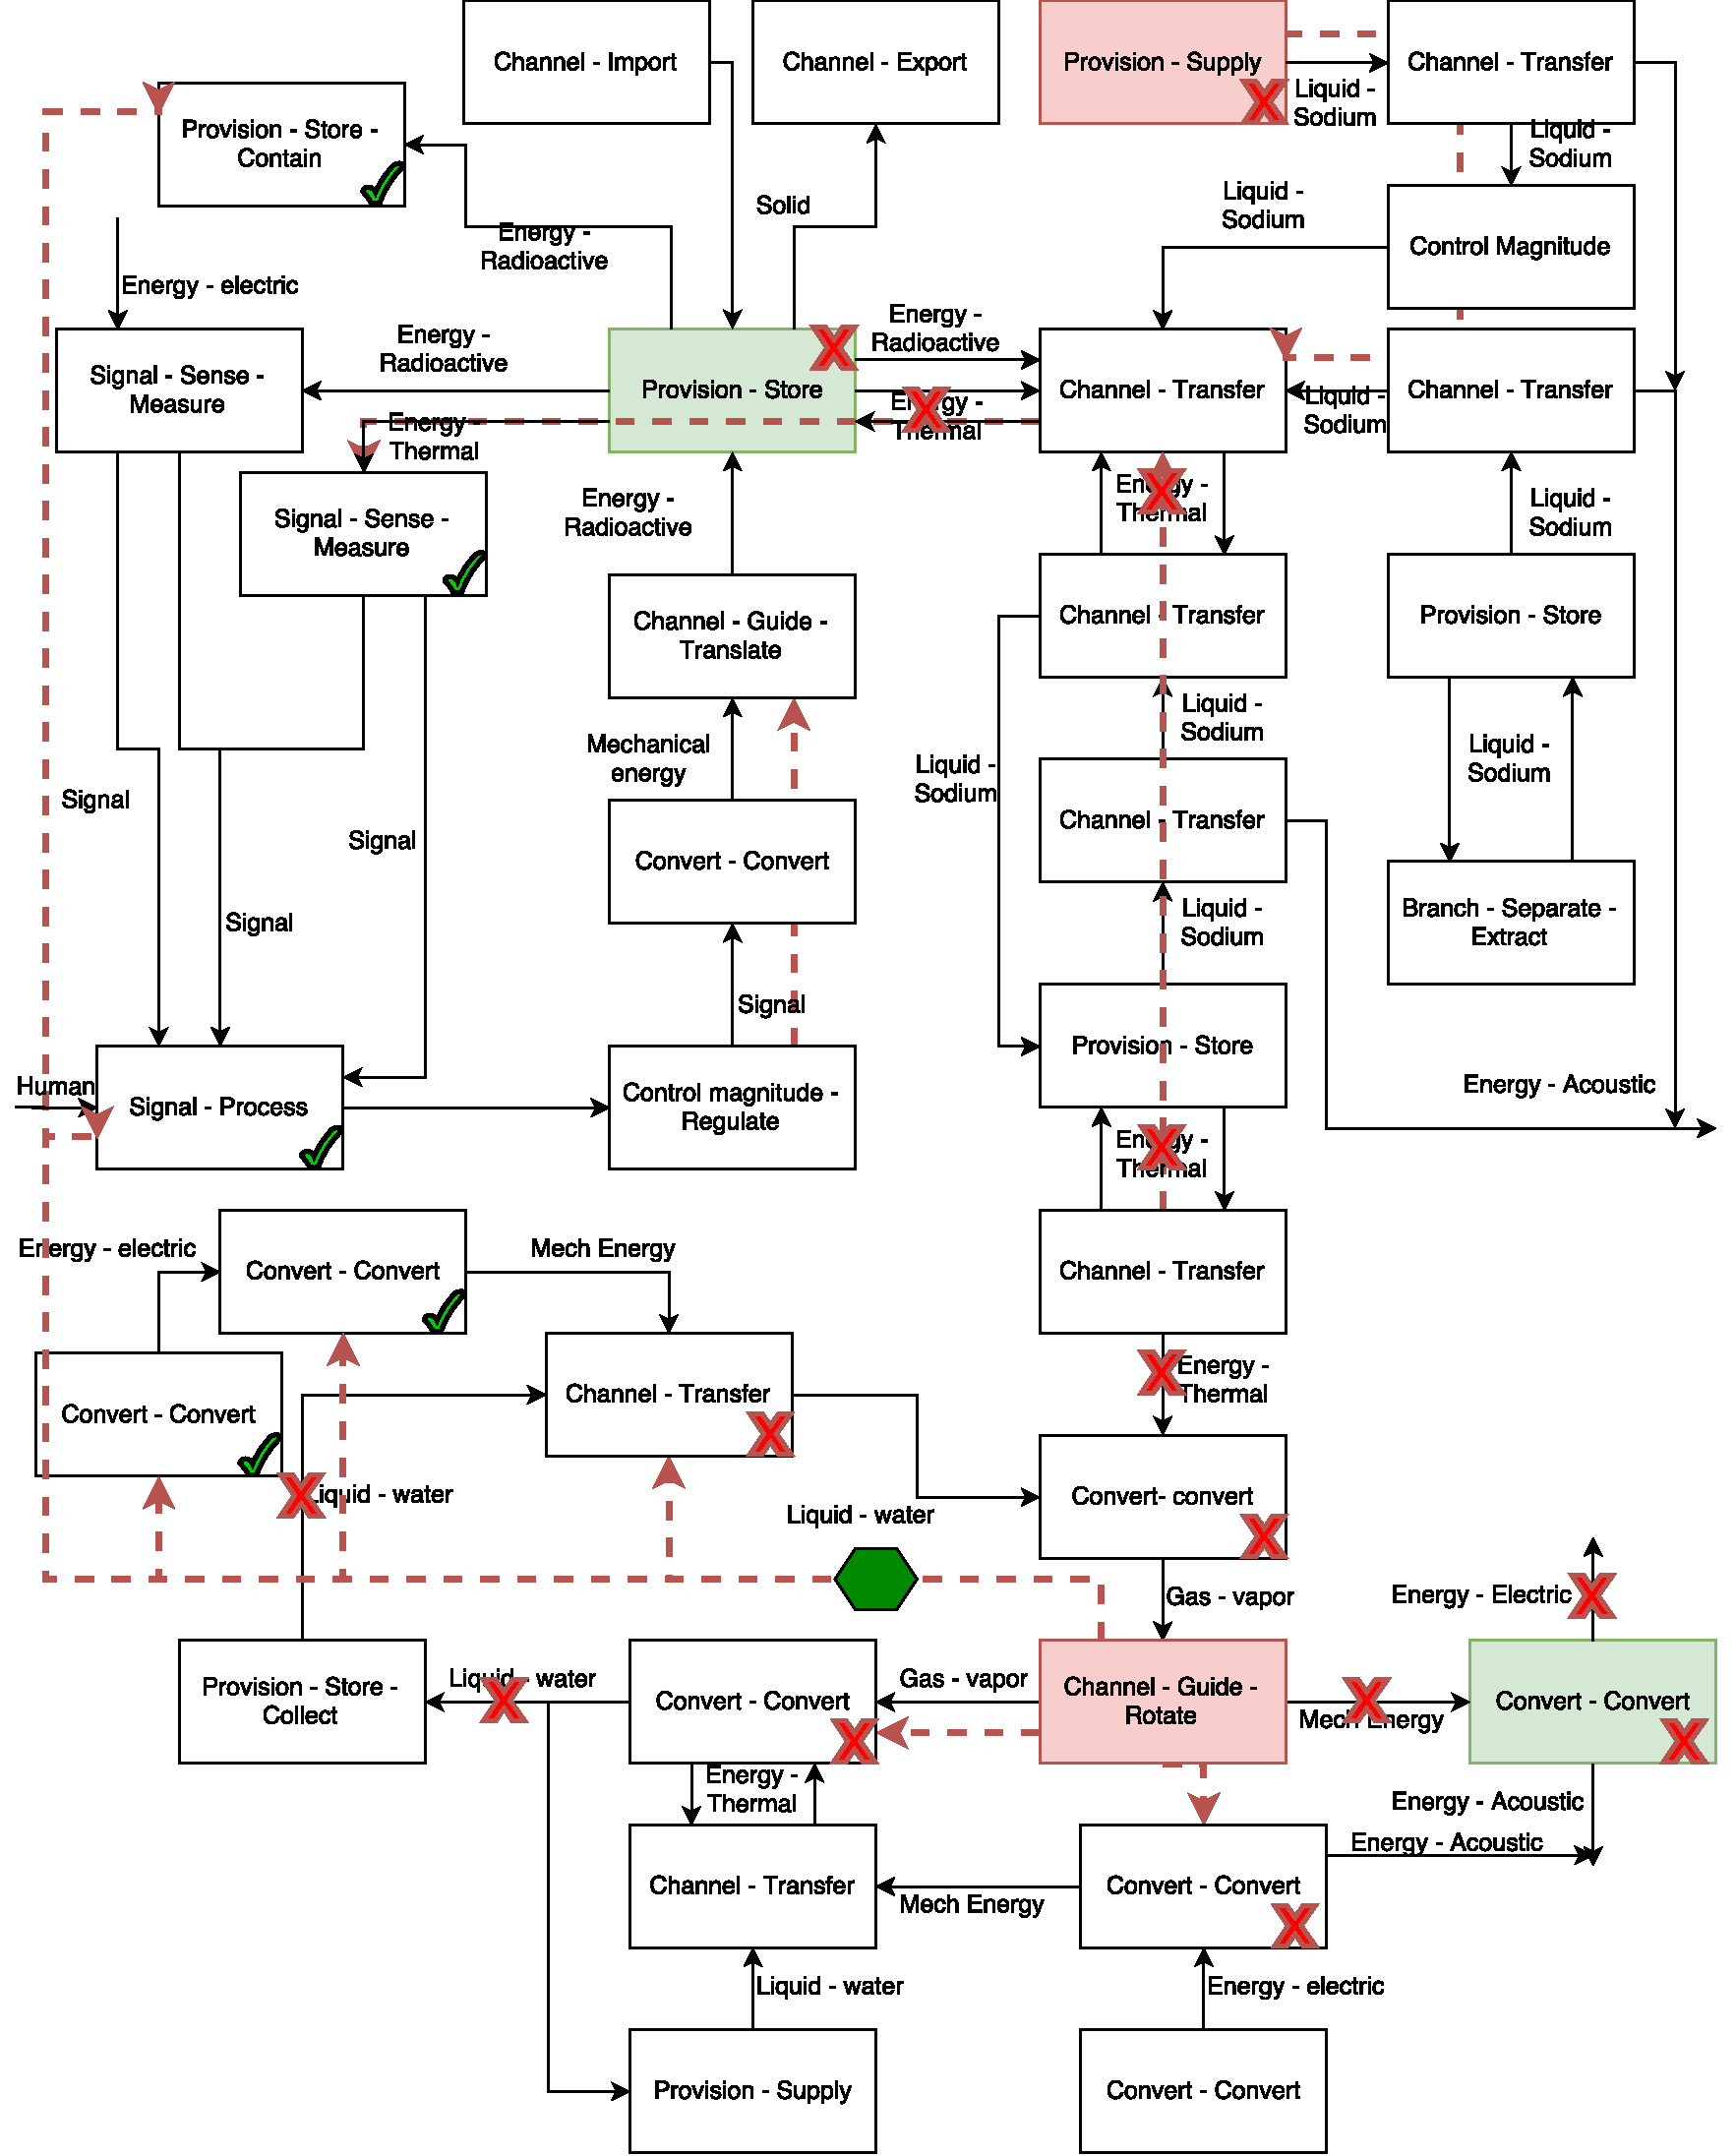
\includegraphics[scale=.55]{fig0e/UFFSR_2}
\caption{UFFSR - Arrestor Function - Initiating event: Turbine explosion - Secondary event: Loss of sodium supply for the SIS}
\label{fig:uffsr2}
\end{figure}


\
